
\subsection{Diffusion Coefficient of Far Field}
\label{sec:diffusivity}

In clay media, diffusion dominates far field hydrogeologic transport due to 
characteristically low hydraulic head gradients and permeability. Thus, the effective diffusion 
coefficient is a parameter to which repository performance in clay media is 
expected to be very sensitive. 

The sensitivity of the peak dose to the reference diffusivity of the 
host rock was analyzed.  In this model, the reference diffusivity of the medium 
was the input parameter used to vary the effective diffusivity in a controlled 
manner. In GoldSim's transport module, the effective diffusion coefficient is 
defined as 

\begin{align}\label{diffcoeff}
  D_{eff} &= n\tau D_{ref}D_{rel} \\ % ?  
       D_{eff} &= ~~\mbox{effective diffusion coefficient }[m^2/s],\nonumber\\
       D_{rel} &= ~~\mbox{relative diffusivity for each isotope in water }[\%],\nonumber\\
       D_{ref} &= ~~\mbox{reference diffusivity in water }[m^2/s],\nonumber\\
       \tau &= ~~\mbox{tortuosity} [\%], \nonumber \\ 
       n &= ~~\mbox{porosity}[\%].\nonumber\\
  \label{GDSEdiff}
\end{align}

The reference diffusivity was altered while the porosity and the tortuosity 
were both set to 1. Thus, the simulation rendered the effective diffusivity 
equal to the product of the reference diffusivity and the relative diffusivity 
(set to 1 for all isotopes).  This allowed the diffusivity to be controlled 
directly for all isotopes.

The waste inventory total mass was also altered for each value of the reference 
diffusivity.  That is, the radionuclide inventory in a reference 
\gls{MTHM} of commercial spent nuclear fuel was multiplied by a scalar mass factor.  
It was expected that changing these two parameters in tandem would capture the 
importance of diffusivity in the far field to the repository performance 
as well as a threshold at which the effect of waste inventory dissolution is 
attenuated by solubility limits.

Finally, in order to isolate the effect of the far field behavior, the waste form 
degradation rate was set to be very high as were the solubility and advective 
flow rate through the  \gls{EBS}. This guaranteed that contaminant flowthrough 
in the near field was unhindered, leaving the far field as the dominant barrier 
to release.


\subsubsection{Parametric Range}
\label{sec:diffCoeffRange}

The forty runs corresponded to eight values of relative diffusivity and five 
values of inventory mass multiplier. That is, the reference diffusivity was varied over the 
eight magnitudes between $ 10^{-8}$ and $10^{-15}$ $[m^2 /s]$ . 
The Mass Factor, the unitless inventory multiplier, was simultaneously varied over 
the five magnitudes between $10^{-4}$ and $10^{1} [-]$. That is, the 
radionuclide inventory was varied between $10^{-4}$ and $10^{1}$ of that in one 
\gls{MTHM} of \gls{SNF}, which is expected to cover the full range of 
inventories in current wasteforms.

\begin{table}[hbp!]
\centering
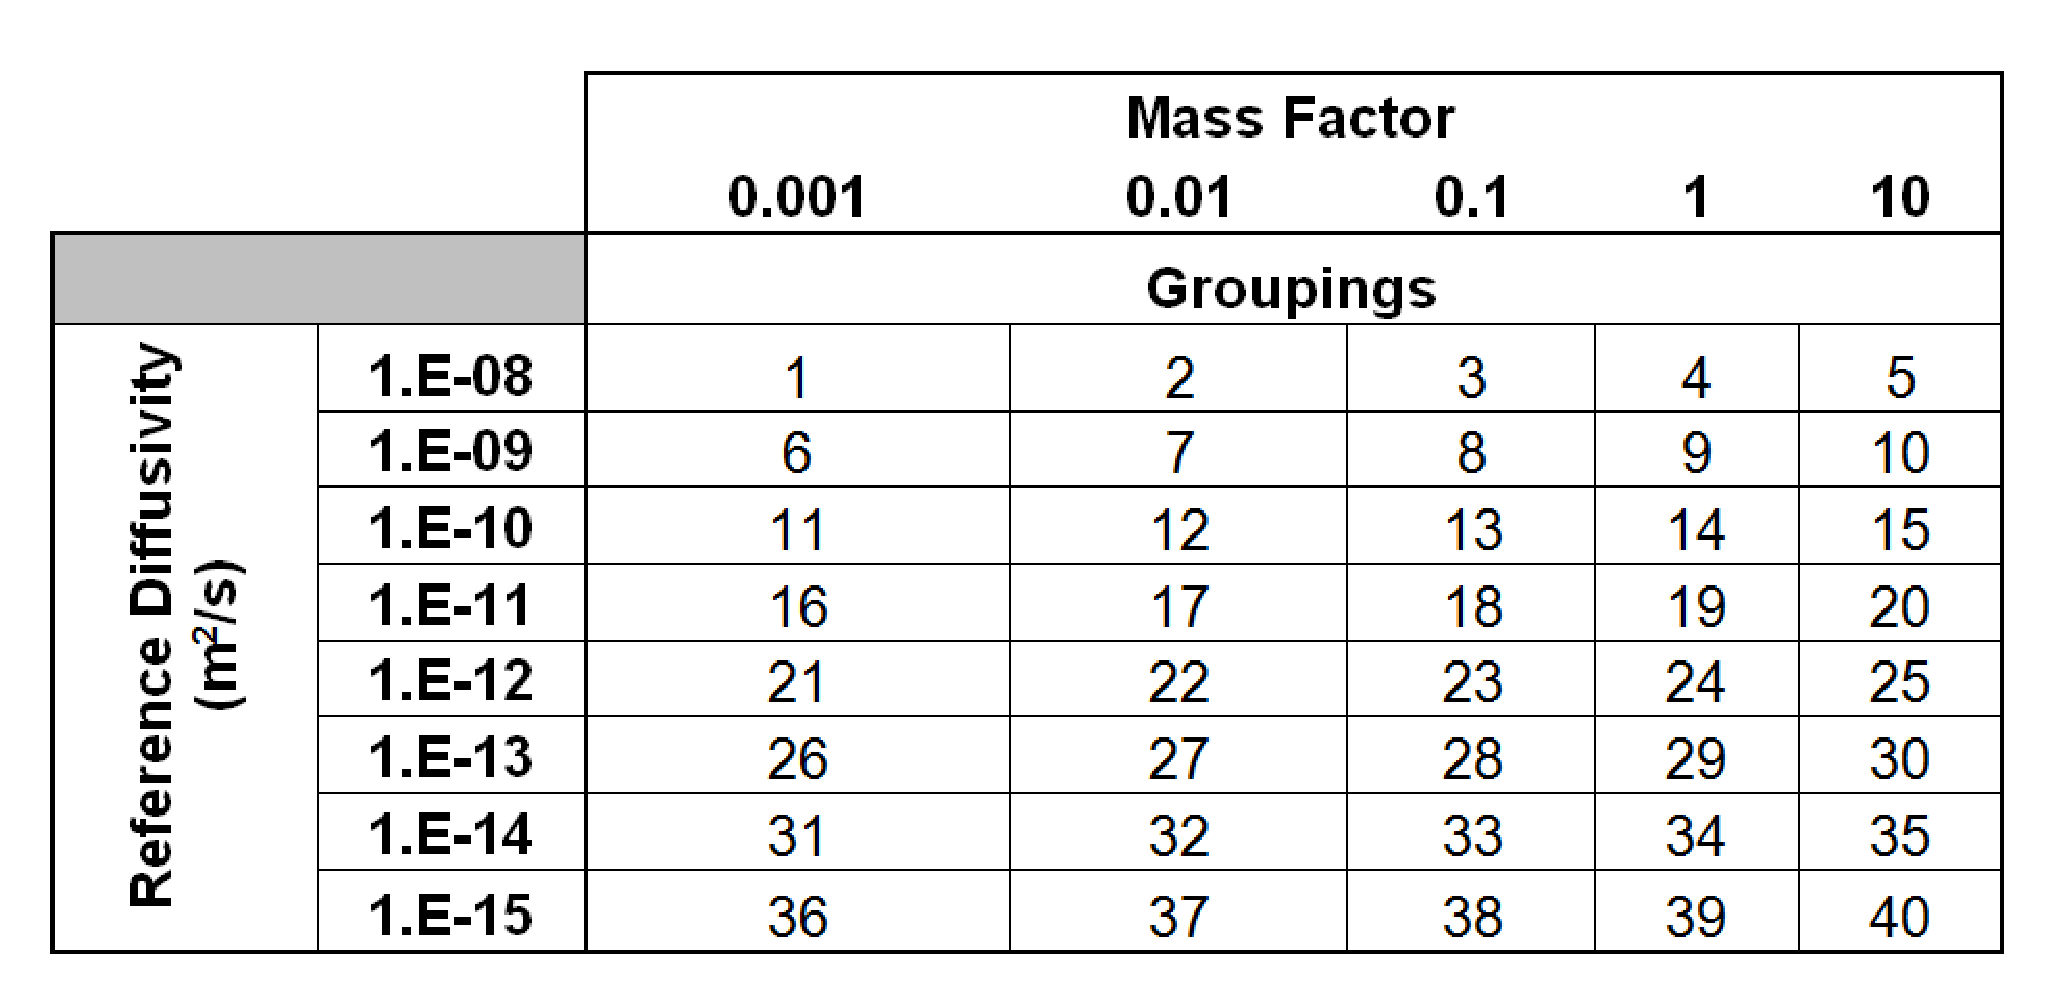
\includegraphics[width=0.7\textwidth]{./chapters/nuclide_sensitivity/clay/DiffCoeffAndInvEBSFail/DiffCoeffAndInvGroups.eps}
\caption{Diffusion coefficient and mass factor simulation groupings.}
\label{tab:DiffCoeffAndInvGroups}
\end{table}


